\documentclass{standalone}
\usepackage{pgfplots}
\pgfplotsset{compat=1.7}

\begin{document}
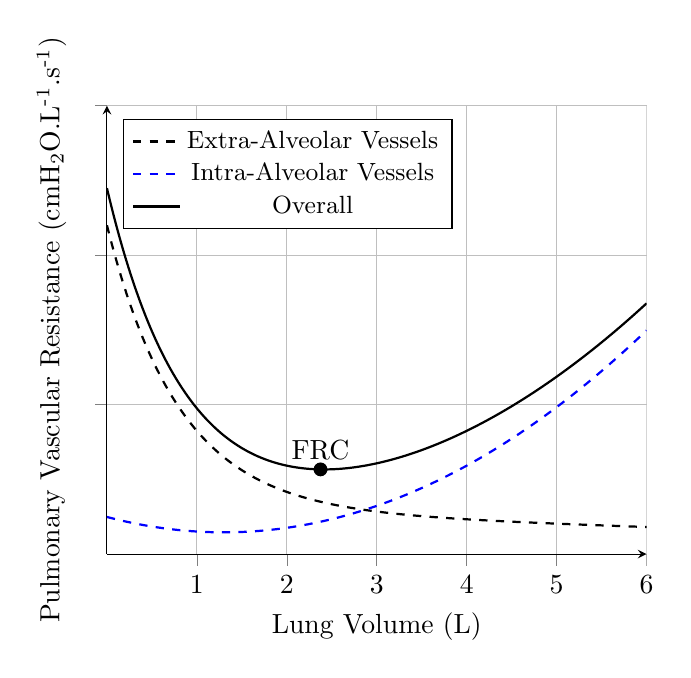
\begin{tikzpicture}


\begin{axis}[
        axis lines=middle,
	ymin = 0,
	ymax = 3,
	xmin = 0,
xmax =6,
yticklabels={},
        grid = major,
	 ylabel near ticks,
	xlabel near ticks,
        xlabel=Lung Volume (L),
        ylabel=Pulmonary Vascular Resistance (cmH\textsubscript{2}O.L\textsuperscript{-1}.s\textsuperscript{-1}),
        tick align=outside,
        enlargelimits=false,
legend pos= north west,
legend style={font=\small, cells={align=left}}]

\plot[domain=0:6, black, dashed, thick,samples=500] {1.9*exp(-1.25*(x)) + 0.3 - 0.02*x};
\addlegendentry{Extra-Alveolar Vessels}
\plot[domain=0:6, blue, dashed, thick,samples=500] {0.2483599 - 0.1585615*x + 0.0611059*x^2};
\addlegendentry{Intra-Alveolar Vessels}

\plot[domain=0:6, black, thick,samples=500] {1.9*exp(-1.25*(x)) + 0.3 - 0.02*x + 0.2483599 - 0.1585615*x + 0.0611059*x^2} node[circle,fill=black,inner sep=0pt,minimum size=5pt, pos=0.46]{} node[pos=0.46, black, above]{FRC};
\addlegendentry{Overall}

\end{axis}

\end{tikzpicture} 
\end{document}